\chapter{Backpropagation}
E' un concetto inizialmente introdotto negli anni 70'. Nel 1986 un articolo di David Rumelhart, Geoffrey Hinton e Ronald Williams mostrò alcune reti neurali in cui la backpropagation lavorava molto più velocemente rispetto agli approcci esistenti; essa \textbf{ha reso possibile la risoluzione di problemi che erano considerati irrisolvibili}.


Oggi l'algoritmo di backpropagation è il vero e proprio cavallo di battaglia delle reti neurali.

\paragraph{Backpropagation vs Discesa del Gradiente.} Abbiamo già visto la discesa del gradiente, quali sono le differenze con la backpropagation?
\begin{itemize}
    \item \textbf{la discesa del gradiente è una procedura generale per l'ottimizzazione di funzioni differenziabili};
    \item \textbf{la backpropagation è un'istanziazione della discesa del gradiente, nel contesto delle reti neurali}.
\end{itemize}
Fornisce i dettagli su come calcolare i gradienti, tiene conto della struttura della rete e risulta computazionalmente efficiente poiché evita di ripetere il calcolo dei gradienti più e più volte.

\section{Notazione}
\paragraph{Matrix based notation.} Useremo $w^l_{jk}$ per denotare il peso dal $k$-esimo neurone al livello $l-1$ verso il $j-$esimo neurone al livello $l$. \textbf{Notare l'ordine degli indici}.
\begin{figure}[!h]
    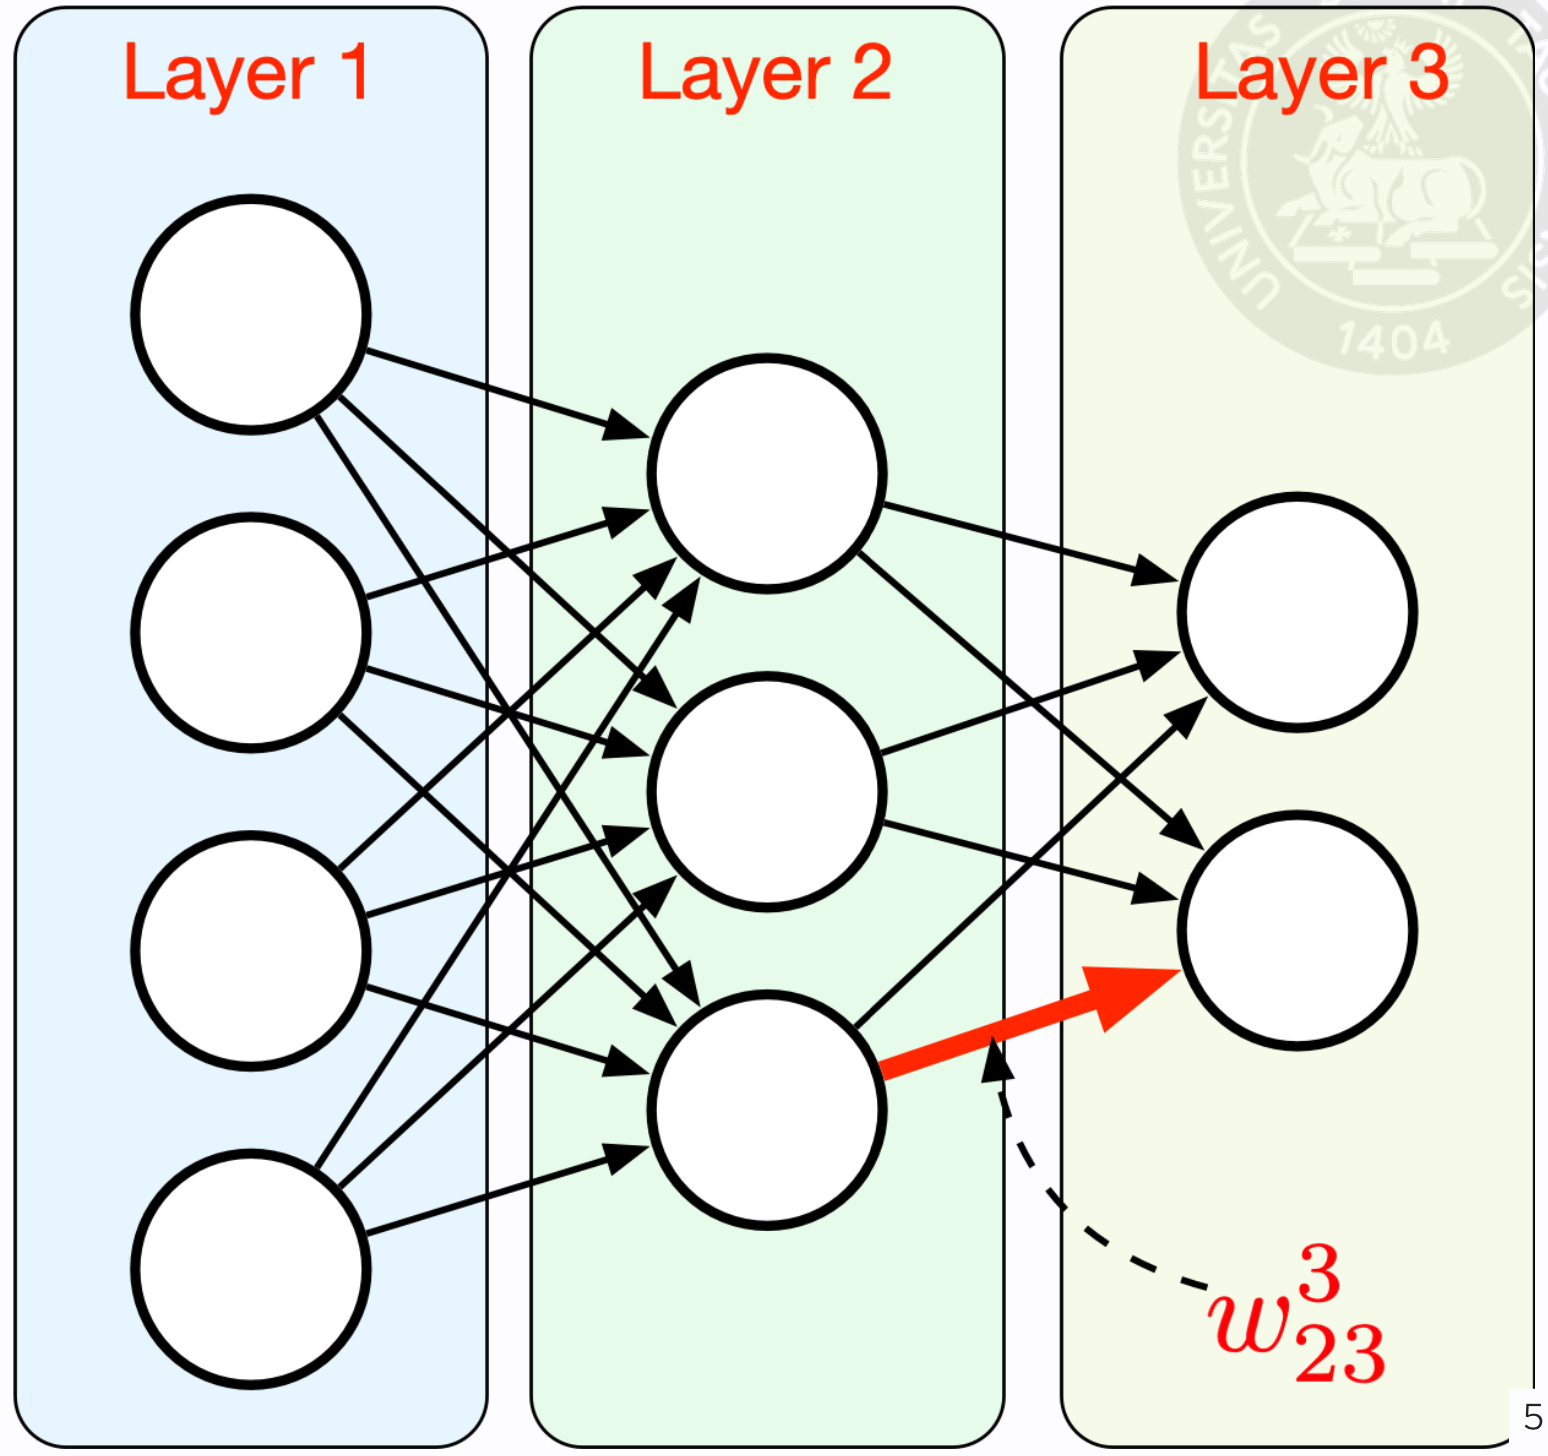
\includegraphics[scale=.33]{images/backpropagation/matrixNotation01.png}
    \centering
\end{figure}
\newpage
Similmente, useremo:
\begin{itemize}
    \item $b_j^l$ per denotare il \textbf{bias} del $j-$esimo neurone nel layer $l$;
    \item $z_j^l$ per denotare il \textbf{valore di attivazione} del $j-$esimo neurone nel layer $l$.
\end{itemize}
\begin{figure}[!h]
    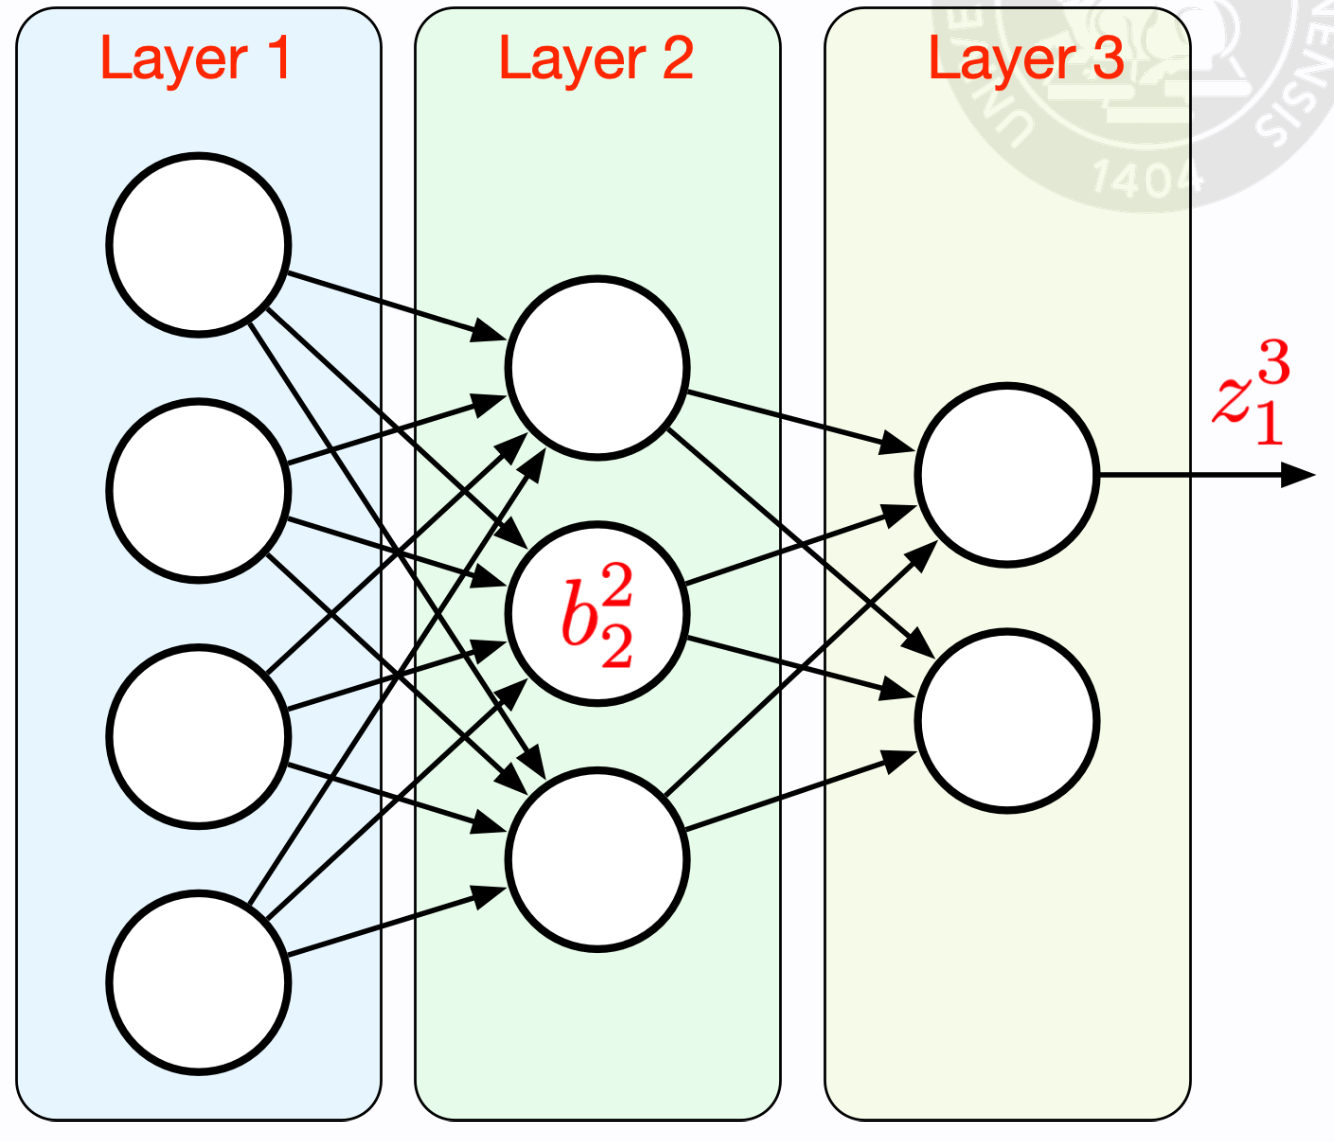
\includegraphics[scale=.4]{images/backpropagation/matrixNotation02.png}
    \centering
\end{figure}


L'attivazione $z_j^l$ del $j-$esimo neurone nel $l-$esimo layer è collegata all'attivazione nel layer $(l-1)$  dall'equazione:
\begin{equation}
    z_j^l=\sigma\Big(\sum_k w^l_{jk} z^{l-1}_k + b_j^l \Big)
\end{equation}
dove la somma è calcolata su tutti i neuroni $k$ del layer $(l-1)$.


Definiamo ancora:
\begin{itemize}
    \item \textbf{W}$^l$ la matrice avente l'elemento $w^l_{jk}$ nella riga $j$ e nella colonna $k$;
    \item $\text{\textbf{b}}^l$ il vettore colonna avente $b_j^l$ come suo $j-$esimo elemento;
    \item \textbf{z}$^l$ il vettore colonna avente $z_j^l$ come suo $j-$esimo elemento;
    \item $f(\textbf{\textbf{v}})$ la versione "fattorizzata" di $f$ se \textbf{v} è un vettore. Per esempio, se $f(x)=x^2$, avremmo:
    \begin{equation}
        f
    \begin{pmatrix}
    \begin{bmatrix}
        2\\
        3
    \end{bmatrix}
    \end{pmatrix}
    =
    \begin{bmatrix}
        f(2)\\
        f(3)
    \end{bmatrix}
    =
    \begin{bmatrix}
        4\\
        9
    \end{bmatrix}
    \end{equation}.
\end{itemize}


Con queste notazioni possiamo calcolare tutto l'insieme delle attivazioni al livello $l$ come:
\begin{equation}
    \text{\textbf{z}}^l=\sigma(\text{\textbf{W}}^l\text{\textbf{z}}^{l-1}+\text{\textbf{b}}^l).
\end{equation}
I vantaggi che ne derivano sono:
\begin{itemize}
    \item è più semplice da scrivere, ragionare e ricordare;
    \item è più semplice da implementare e il risultato è più veloce da calcolare (traendo vantaggio dalle librearie numeriche per il calcolo delle operazioni tra matrici).
\end{itemize}
\newpage
Per semplificare la notazione futura, definiamo l'input pesato del neurone al livello $l$ come $a_l$:
\begin{equation}
    \text{\textbf{a}}^l\equiv\text{\textbf{W}}^l\text{\textbf{z}}^{l-1}+\text{\textbf{b}}^l
\end{equation}
questa scrittura:
\begin{itemize}
    \item ci permette di scrivere gli output al livello $l$ semplicemente come $\text{\textbf{z}}^l=\sigma(\text{\textbf{a}}^l)$;
    \item implica che il componente $j$ del vettore \textbf{a}$^l$ sia $a_j^l=\sum_k w_{jk}^l z^{l-1}_k + b_j^l$.
\end{itemize}

\subsection{Assunzioni sulla funzione costo} Per far si che l'algoritmo di backpropagation funzioni, abbiamo bisogno di fare alcune assunzioni sulla funzione costo. Nello specifico, assumeremo che:
\begin{itemize}
    \item possa essere scritta come la una media $C=\frac{1}{n}\sum_\text{\textbf{x}}C_\text{\textbf{x}}$ della fuznione costo $C_\text{\textbf{x}}$ per singoli esempi di training, \textbf{x};
    \item sia una funzione degli output della rete neurale.
\end{itemize}

Come esempio, è semplice vedere come entrambe le assunzioni siano soddisfatte dalla funzione di costo quadratica, introdotta precedentemente:
\begin{equation}
    C=\frac{1}{2n}\sum_\text{\textbf{x}}\|\text{\textbf{y}}(\text{\textbf{x}}-\text{\textbf{z}}^L(\text{\textbf{x}}))\|^2.
\end{equation}
Se chiamiamo l'espressione $\|\text{\textbf{y}}(\text{\textbf{x}}-\text{\textbf{z}}^L(\text{\textbf{x}}))\|^2 = C_\text{x}$, essa  equivale all'espressione della prima delle due assunzioni che abbiamo fatto.

\paragraph{Prodotto di Hadamard.} Nel seguito, assumeremo la familiarità sulle operazioni standard tra matrici (somma, sottrazioni, prodotto ecc.). Un operatore usato in maniera meno comune è il \textbf{prodotto di Hadamard}.


\textbf{Definizione:} dati due vettori \textbf{s} e \textbf{t}, il prodotto di Hadamard tra i due (scritto $\text{\textbf{s}}\odot\text{\textbf{t}}$) è semplicemente il prodtto degli elementi dei due vettori, cioè le componenti di $\text{\textbf{s}}\odot\text{\textbf{t}}$ sono semplicemente ($\text{\textbf{s}}\odot\text{\textbf{t}})=s_jt_j$.
Per esempio:
\begin{equation}
    \begin{bmatrix}
        1\\
        2
    \end{bmatrix}
    \odot
    \begin{bmatrix}
        3\\
        4
    \end{bmatrix}
    =
    \begin{bmatrix}
        1\cdot 3\\
        2\cdot 4
    \end{bmatrix}
    =
    \begin{bmatrix}
        3\\
        8
    \end{bmatrix}
\end{equation}
\newpage
\section{Backpropagation: le quattro equazioni fondamentali}
Per sviluppare la comprensione dell'algoritmo di backpropagation, miriamo allo studio su come calcolare in modo efficiente le quantità $\frac{\partial C}{\partial w^l_{jk}}$ e $\frac{\partial C}{\partial b^l_{j}}$.


Sembra essere più facile farlo, calcolando prima un'altra quantità:
\begin{equation}
    \delta^l_j=\frac{\partial C}{\partial a^l_{j}}.
\end{equation}
Ci riferiremo a $\delta^l_j$ come l'errore al livello $l$ e neurone $j$. %?


La backpropagation ci da una procedura per il cacolo di $\delta_j^l$per ogni layer $l$ e neurone $j$, e lega $\delta_j$ alla quantità di reasle interesse.

\paragraph{Significato di $\textbf{$\delta^l$}$.} L'errore al livello $l$ dovrebbe misurare la variazione della funzione costo in quando gli input dei neuroni a quel livello sono leggermente perturbati. Il termine "errore" deriva dell'idea di introdurre un piccolo "errore" negli input del layer e osservare come esso si propaga alla funzione costo.

\paragraph{Le quattro equazioni fondamentali.} L'algoritmo di backpropagation è basato sulle \textit{quattro equazioni fondamentali}. Le introdurremo inizialmente senza una prova, concentrandoci sul loro significato. In seguito mostreremo come derivarle dai primi principi.
\newline
\newline
\subsection{Un'equazione per l'errore dell'ouput layer}
L'equazione \textit{BP1} specifica come calcolare $\delta^L$, cioè l'errore del layer di output (\textit{L} indica appunto il layer di output):
\begin{equation}
    \delta^L=\frac{\partial C}{\partial z^L_j}\sigma'(a^L_j).
\end{equation}
\paragraph{Interpretazione}
\begin{itemize}
    \item $\delta^L_j=\frac{\partial C}{\partial z^L_j}\sigma'(a^L_j)$, $\delta^L_j$ è la derivata della funzione costo rispetto a $z_j^L$ moltiplicata per la derivata della funzione di schiacciamento calcolata in $a^L_j$. Ci stiamo chiedendo quanto $C$ cambia al variare del peso $z^L_j$;
    \item $z_j^l=\sigma(a^L_j)$.
\end{itemize}
\begin{figure}[!h]
    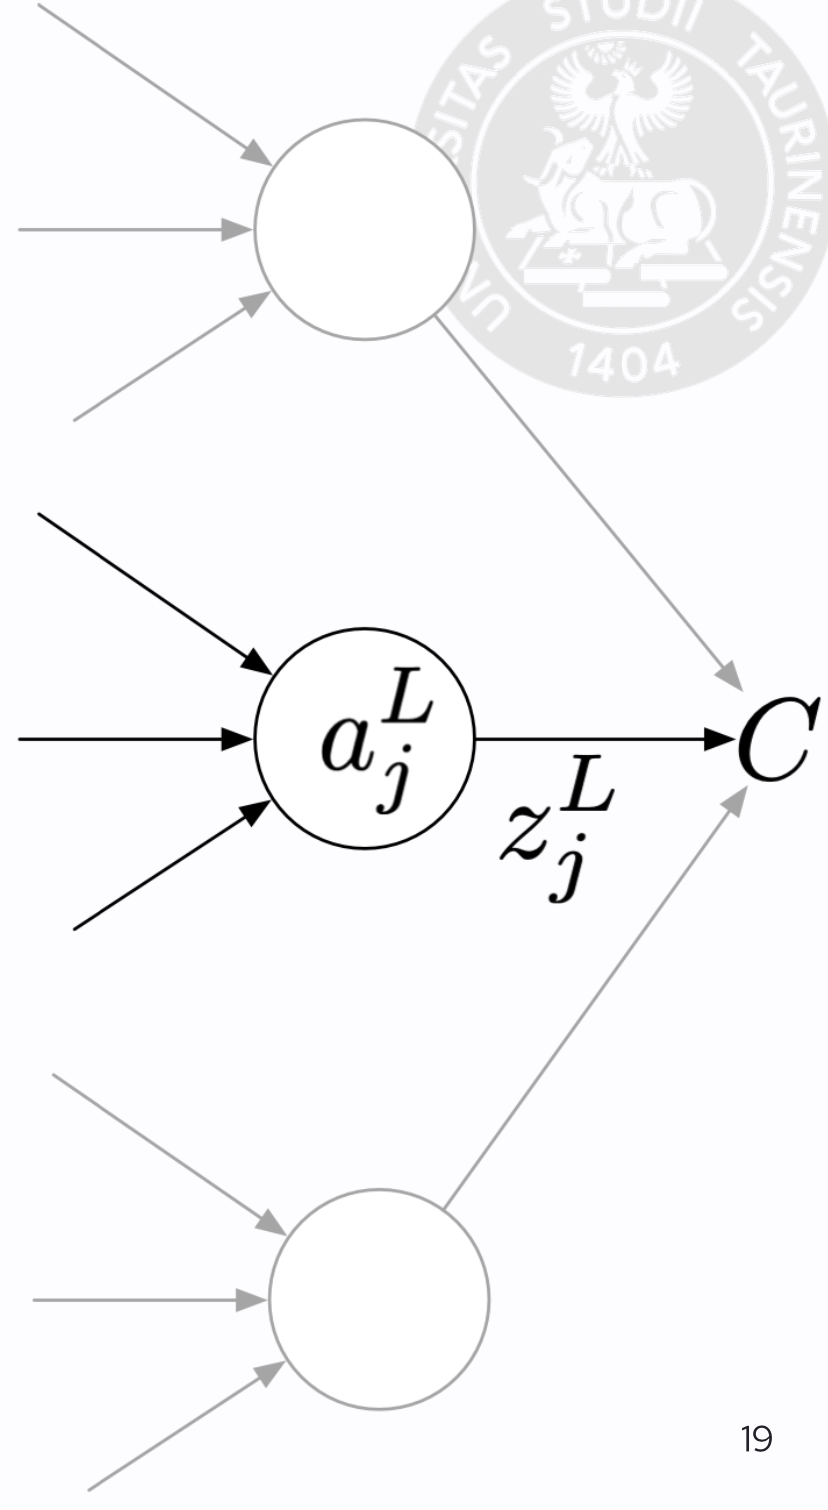
\includegraphics[scale=.25]{images/backpropagation/firstEq.png}
    \centering
\end{figure}
\newpage
\begin{equation}
    \delta^L=\frac{\partial C}{\partial z^L_j}\sigma'(a^L_j).
\end{equation}

Notare che tutto nelle \textit{BP1} è facilmente calcolabile. $a_j^L$ è facilmente calcolabile semplicemente lasciando fluire gli input attraverso la rete verso il neurone $j$ al livello $L$ ed è poi molto facile anche calcolare $\sigma'(a^L_j)$.



L'esatta forma di $\frac{\partial C}{\partial z_j^L}$ dipendere dalla forma della funzione costo. 


Per esempio, se il costo è quadratico, allora:
\begin{equation}
    C_x=\frac{1}{2}\sum_j(y_j - z^L_j)^2\Rightarrow \frac{\partial C}{\partial z^L_j} = (z^L_j - y_j).
\end{equation}
Il termine $\frac{1}{2}\sum_j(y_j - z^L_j)^2$ deriva da:
\begin{equation}
    \frac{1}{2}\|y(x)-z^L(x)\|^2_2=
    \frac{1}{2}[y(x)-z^L(x)]^T[y(x)-z^L(x)]=\frac{1}{2}\sum_j(y_j(x)-z^L(x))(y_j(x)-z^L(x))
\end{equation}
la quale è esattamente uguale a:
\begin{equation}
    \frac{1}{2}\sum_j(y_j(x)-z^L(x))(y_j(x)-z^L(x))=\frac{1}{2}\sum_j(y_j - z^L_j)^2.
\end{equation}
La parte interessante arriva ora, perchè devo fare la derivata di questo termine. Devo calcolare la derivata parziale della funzione costo rispetto a $z^L_j$.
\begin{equation}
    \frac{1}{2}\Big((y_1-z^L_1)^2+(y_2-z^L_2)^2\cdots(y_j-z^L_j)^2\cdots\Big).
\end{equation}
Sostanzialmente tutti i fattori sono costanti rispetto ad $z^L_j$ ad eccezione di $(y_j-z^L_j)^2$ che è una funzione. Ora, vogliamo la derivata:
\begin{equation}
    \frac{\partial}{\partial z^L_j} (j_j-z^L_j)^2=2(j_j-z^L_j)-1=2(z_j^L-y_j)
\end{equation}
da qui, il $2$ si semplifica con $\frac{1}{2}$ del passaggio precedente e rimaniamo con
\begin{equation}
    (z^L_j - y_j).
\end{equation}



Data l'espressione $\delta^L_j=\frac{\partial C}{\partial z^L_j}\sigma'(a^L_j)$, non dovrebbe essere difficile vedere che l'intero $\delta^L$ può essere scritto come:
\begin{equation}
    \delta^L=\nabla_\text{\textbf{z$^L$}}C\odot\sigma'(\text{\textbf{a}}^L).
\end{equation}
Dove $\nabla_\text{\textbf{z}}C$ è il vettore le cui componenti sono le derivate parziali $\frac{\partial C}{\partial z^L_j}$.
\newpage
\subsection{Un'equazione per $\delta^l$ in termini di $\delta^{l+1}$}
L'equazione \textit{BP2} specifica come calcolare l'errore al livello $l$ in termini dell'errore al livello $l+1$:
\begin{equation}
    \delta^l=((\text{\textbf{W}}^{l+1})^T\delta^{l+1})\odot\sigma'(\text{\textbf{a}}^l).
\end{equation}
\paragraph{Interpretazione}
\begin{itemize}
    \item $ \delta^l=((\text{\textbf{W}}^{l+1})^T\delta^{l+1})\odot\sigma'(\text{\textbf{a}}^l)$;
    \item un termine misura quanto velocemente l'output a questo livello variano in risposta alla variazione del suo input: $\sigma'(\text{\textbf{a}}^l)$;
    \item multiplicato per un termine che misura come questi cambiamento si propaga attraverso la rete utilizzando i pesi connessi: $(\text{\textbf{W}}^{l+1})^T$;
    \item moltiplicato per quanto velocemente quel livello cambia in risposta al cambiamento del suo input.
\end{itemize}
\begin{figure}[!h]
    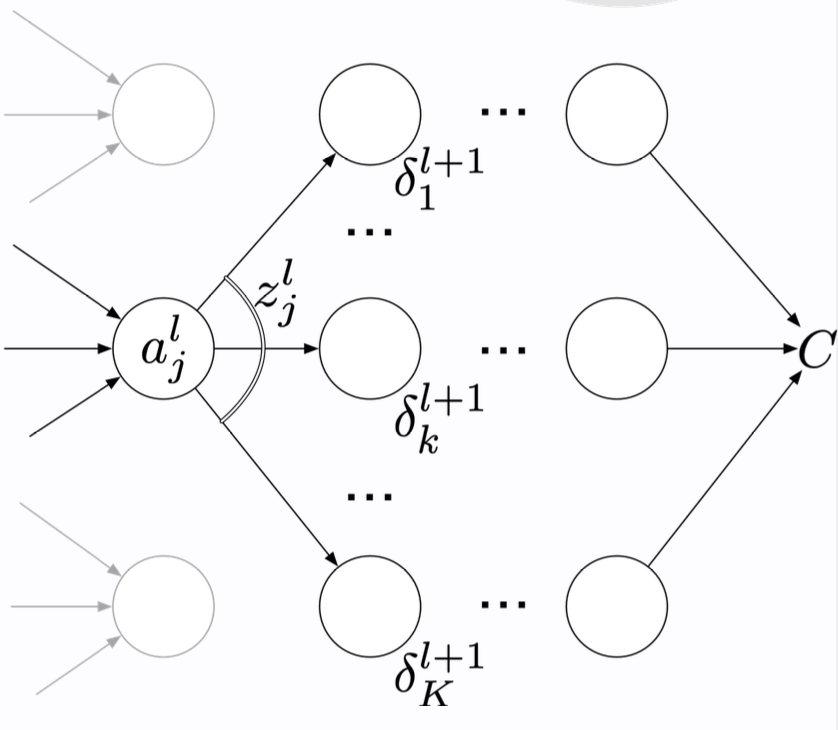
\includegraphics[scale=.4]{images/backpropagation/secondEq.png}
    \centering
\end{figure}

Di nuovo, tutto in questa espressione
\begin{equation}
    \delta^l=((\text{\textbf{W}}^{l+1})^T\delta{l+1})\odot\sigma'(\text{\textbf{a}}^l).
\end{equation}
è facilmente calcolabile in quanto l'unico termine non triviale, cioè $\delta^{l+1}$, può essere calcolato applicando l'equazione \textit{BP1} all'ultimo livello della rete e poi l'equazione \textit{BP2} fino al raggiungimento del livello a cui siamo interessati.
\newpage
\subsection{Un'equazione per il tasso di variazione del costo rispetto ai bias nella rete}
\textit{BP3}: questa è la prima delle due equazioni a cui siamo \textbf{veramente interessati}. Infatti, queste sono le equazioni direttamente collegate all'applicazione della discesa del gradiente ad una rete neurale.
\begin{equation}
    \frac{\partial C}{\partial b_j^l}=\delta^l_j,
\end{equation}
in cui $\delta^l_j$ è \textbf{esattamente uguale} al tasso di cambiamento $\frac{\partial C}{\partial b_j^l}$.
\subsection{Un'equazione per il tasso di variazione del costo rispetto ai pesi nella rete}
\textit{BP4} specifica come calcolare il tasso di variazione del costo (la derivata della funzione costo) rispetto ai pesi nella rete:
\begin{equation}
    \frac{\partial C}{\partial w_{jk}^l}=z_k^{l-1}\delta_j^l,
\end{equation}
la quale può anch eessere scritta in una forma più compatta come:
\begin{equation}
    \frac{\partial C}{\partial w}=z_{in}\delta_{out},
\end{equation}
dove si intende che il peso $w$ rispetto al quale stiamo prendendo la derivata determini il livello e l'indice di $z_{in}$ e $\delta_{out}$.

\paragraph{Consequenze delle equazioni \textit{BP1-BP4}.} Cerchiamo ora di capire quali siano le conseguenze di queste 4 equazioni, a partire da \textit{BP4}:
\begin{equation}
    \frac{\partial C}{\partial w}=z_{in}\delta_{out},
\end{equation}
notiamo che implica che ovunque $z_{in}$ sia piccola, il gradiente tende anche lui ad essere piccolo e l'apprendimento di quel peso sarà lento. In altre parole, i pesi orginati da \textbf{unità a bassa attivazione (low activation units)} si evolveranno lentamente. 
\newline
\newline
Consideriamo ora l'equazione \textit{BP1}:
\begin{equation}
    \delta^L=\frac{\partial C}{\partial z^L_j}\sigma'(a^L_j)
\end{equation}
ed in particolare il termine $\sigma'(a^L_j)$. Il grafico della funzione sigmoide mostra che la sua derivata è quasi zero quando il suo argomento è o molto grande o molto piccolo.


Cioè, il processo di apprendimento procederà lentamente per l'output di un neurone sia che abbia bassa attivazione ($\approx 0$) sia che abbia alta attivazione ($\approx 1$)


Quando la derivata della funzione di attivazione è quasi zero è comune dire che il neurone \textbf{si è saturato}.
\newline
\newline
La generalità delle osservazioni riguardo \textit{BP1-BP4} mostra che possiamo usare queste intuizioni per creare nuove funzioni di attivazione che abbiano particolari proprietà di apprendimento che desideriamo.


Come esempio, supponiamo che dovessimo scegliere una (non sigmoide) funzione di attivazione $\sigma$ tale che $\sigma'$ sia sempre positiva e non si avvicini mai a zero.


Ciò impedirebbe il rallentamento del processo di apprendimento che avviene quando normali neuroni sigmoidi si saturano.
\newpage
\subsection{Sommario: le equazioni della backpropagation}
\begin{itemize}
    \item \textit{(BP1):}$\delta^L=\nabla_\textbf{z}\sigma'(a^L_j)$;
    \item \textit{(BP2):}$\delta^l=((\text{\textbf{W}}^{l+1})^T\delta^{l+1})\odot\sigma'(\text{\textbf{a}}^l)$;
    \item \textit{(BP3):}$\frac{\partial C}{\partial b_j^l} = \delta_j^l$;
    \item \textit{(BP4):}$\frac{\partial C}{\partial w_{jk}^l} = z^{l-1}_k\delta^l_j$.
\end{itemize}
\newpage
\section{Prove della solidità delle 4 equazioni fondamentali}
Vediamo ora come derivare \textit{BP1} da \textit{BP4}. In questo frangente faremo pesante uso della \textbf{chain rule per il calcolo multivariato}. Essa afferma che se $f$ è una funzione di $g$ e $h$, le quali a loro volta sono funzioni di $x$, cioè $f(x)=f(g(x),h(x))$ allora:
\begin{equation}
    \frac{\partial f}{\partial x} = \frac{\partial f}{\partial g} \frac{\partial g}{\partial x} + \frac{\partial f}{\partial h} \frac{\partial h}{\partial x}.
\end{equation}
\subsection{Dimostrazione di \text{BP1}}
Vogliamo dimostrare che
\begin{equation}
    \delta^L_j \equiv \frac{\partial C}{\partial a^L_j} = 
    \frac{\partial C}{\partial z^L_j}\sigma'(a^L_j)
\end{equation}
\begin{figure}[!h]
    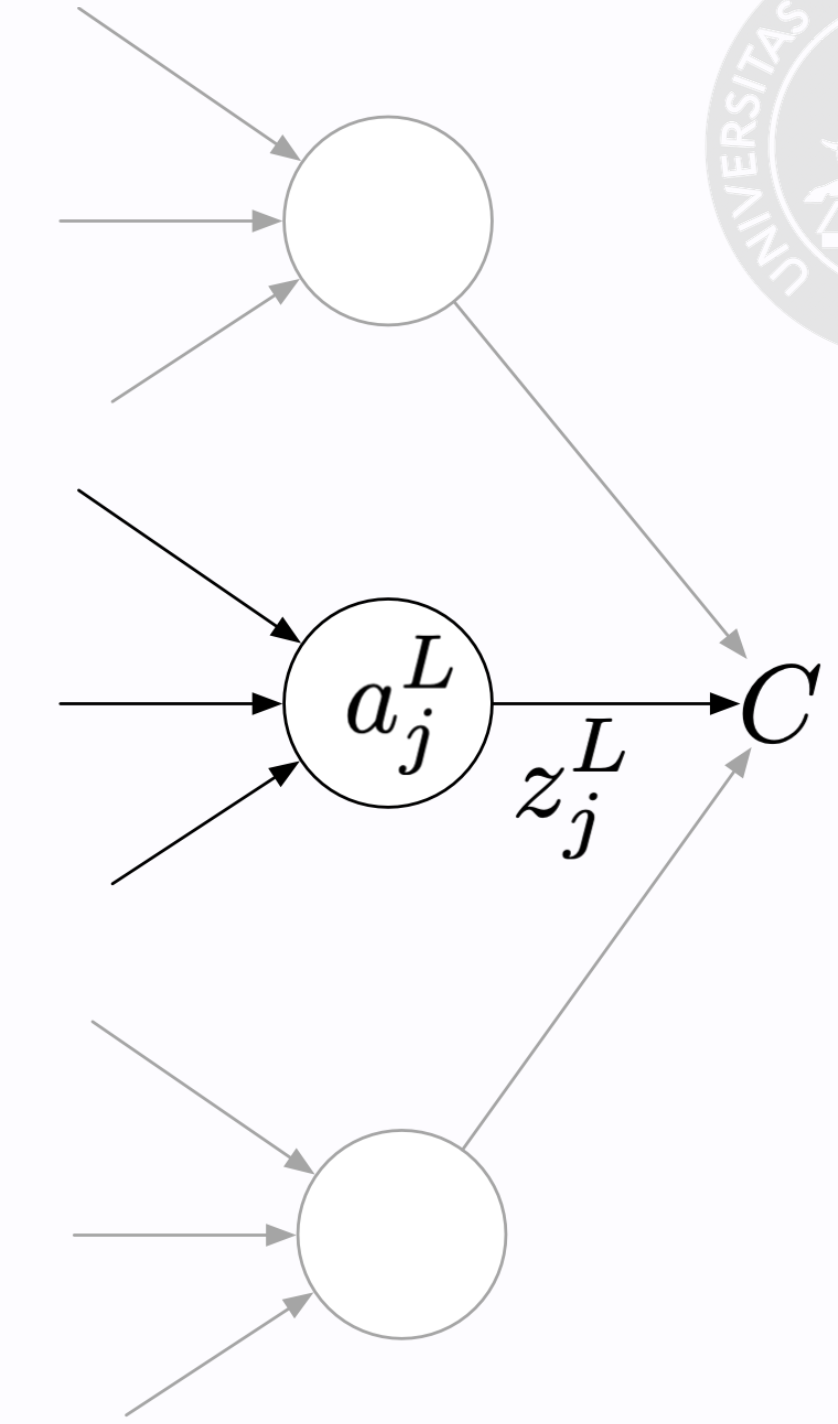
\includegraphics[scale=.3]{images/backpropagation/proofBp1.png}
    \centering
\end{figure}


Sfruttando il fatto che $C$ è una funzione di tutti gli output $z^L_j$ e applicando la chain rule per il calcolo multivariato, otteniamo:
\begin{equation}
    \delta^L_j=\frac{\partial C}{\partial a^L_j}=\sum_k\frac{\partial C}{\partial z^L_k}\frac{\partial z^L_k}{\partial a^L_j}.
\end{equation}
Ma dato che solo $z^L_j$ dipende da $a^L_j$, tutti i termini ad eccezione di uno valgono zero, quindi:
\begin{equation}
    \delta^L_j = \frac{\partial C}{\partial a^L_j} = \frac{\partial C}{\partial z^L_j} \frac{\partial z^L_j}{\partial a^L_j} = \frac{\partial C}{\partial z^L_j}\sigma'(a^L_j)
\end{equation}
dove l'ultima uguaglianza deriva da $z^L_j = \sigma(a^L_j)$.
\newpage
\subsection{Dimostrazione di \text{BP2}}
Vogliamo dimostrare che
\begin{equation}
    \delta^l_j = \frac{\partial C}{\partial a^l_j} = \big( (\text{\textbf{W}}^{l+1})^T \delta^{l+1} \odot \sigma'(a^l) \big)_j =
    \sum_kw_{kj}^{l+1}\delta^{l+1}_k\sigma'(a^l_j).
\end{equation}
\begin{figure}[!h]
    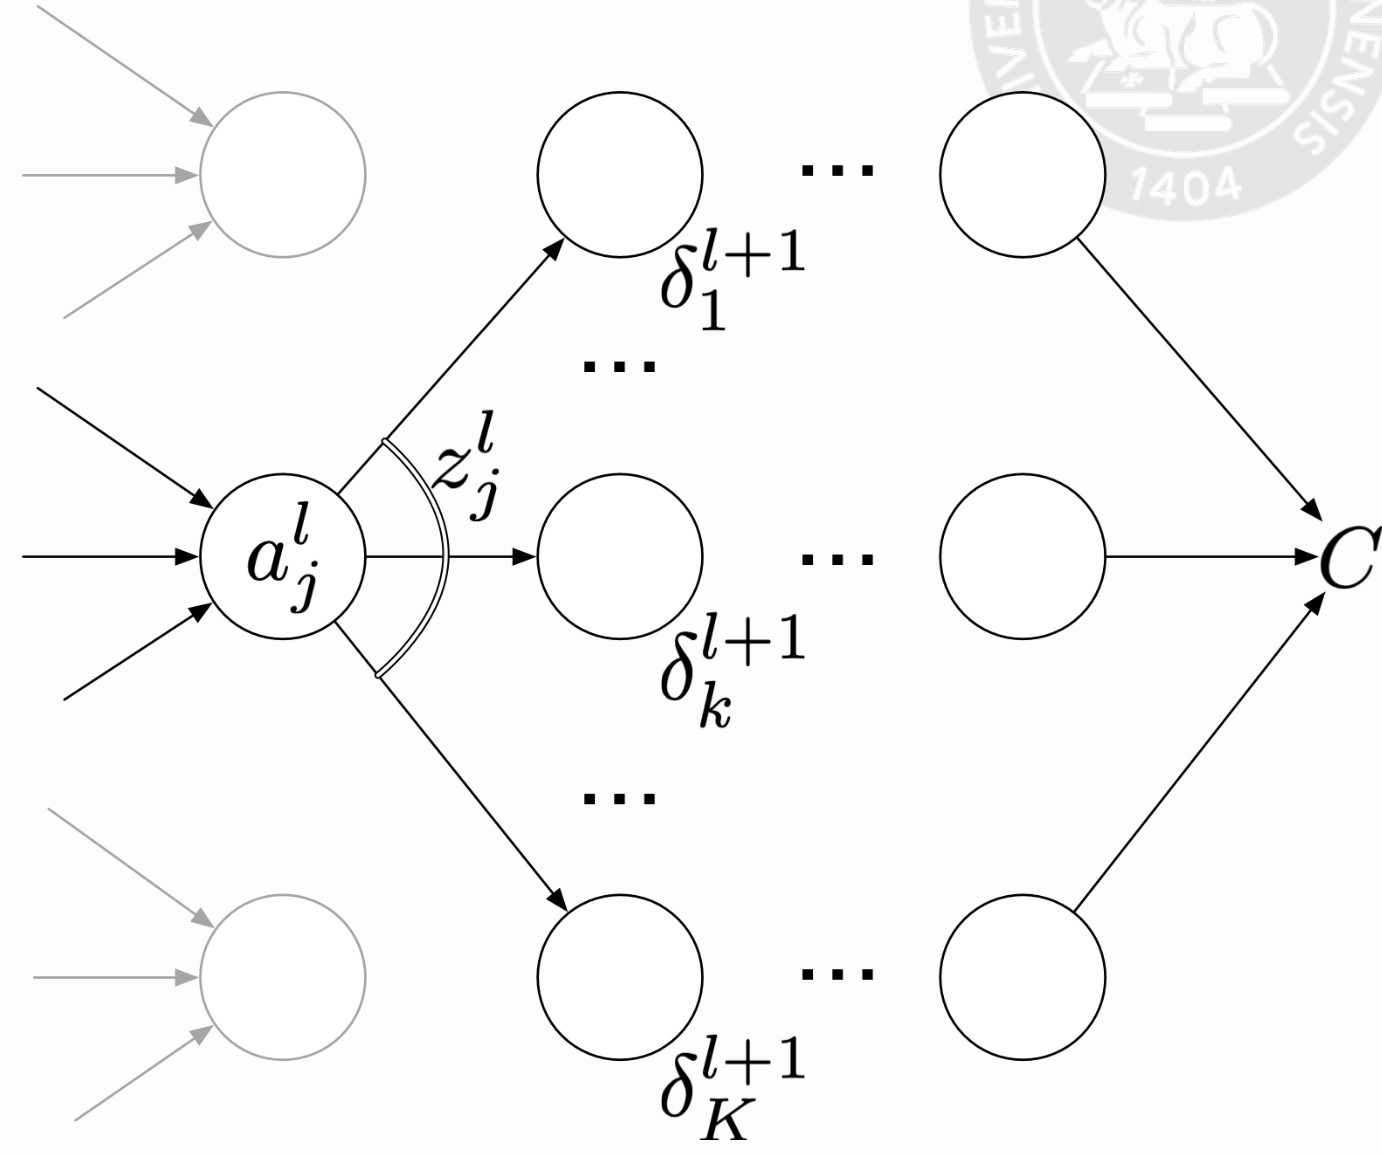
\includegraphics[scale=.3]{images/backpropagation/proofBp2.png}
    \centering
\end{figure}

Cominciamo riscrivendo $\delta^l_j$ in termini di $\delta^{l+1}_k$. Di nuovo, sfruttiamo la chain rule osservando che $C$ può essere vista come una funzione di $a^{l+1}_k$ la quale, a sua volta, può essere vista come una funzione di $a^l_j$.
\begin{equation}
    \delta^l_j = \frac{\partial C}{\partial a^l_j} = \sum_k\frac{\partial C}{\partial a^{l+1}_k}\frac{\partial a_k^{l+1}}{\partial a^l_j}.
\end{equation}
Notiamo ora che, per definizione, $\frac{\partial C}{\partial a^{l+1}_k} = \delta_k^{l+1}$, quindi:
\begin{equation}
    \delta^l_j = \sum_k\frac{\partial a_k^{l+1}}{\partial a^l_j}\delta^{l+1}_k.
\end{equation}
Ora ricordiamo che:
\begin{equation}
    a^{l+1}_k = \sum_jw^{l+1}_{kj}z^l_j+b^{l+1}_k = \sum_jw^{l+1}_{kj}\sigma(a^l_j)+b^{l+1}_k
\end{equation}
ciò implica:
\begin{equation}
    \frac{\partial a_k^{l+1}}{\partial a^l_j} = w^{l+1}_{kj}\sigma'(a^l_j).
\end{equation}
Mettendo tutto insieme abbiamo:
\begin{equation}
    \delta^l_j = \sum_kw^{l+1}_{kj}\sigma'(a^l_j)\delta^{l+1}_k = \sum_kw^{l+1}_{kj}\delta^{l+1}_k\sigma'(a^l_j)
\end{equation}

\newpage
\subsection{Dimostrazione di \textit{BP3}}
Vogliamo dimostrare che
\begin{equation}
    \frac{\partial C}{\partial b^l_j} = \delta^l_j.
\end{equation}

Cominciamo di nuovo interpretando $C$ come una funzione di $a^l_j$ e applicando la chain rule del caso multivariato:
\begin{equation}
    \frac{\partial C}{\partial b^l_j} = \sum_k \frac{\partial C}{\partial  a^l_k}\frac{\partial a^l_k}{\partial b^l_j}.
\end{equation}
Notiamo che l'unico $a^l_k$ che dipende da $b^l_j$ è $a^l_j$, possiamo semplificarlo come 
\begin{equation}
    \frac{\partial C}{\partial b^l_j} = \frac{\partial C}{\partial a^l_j}\frac{\partial a^l_j}{\partial b^l_j} = \delta^l_j\frac{\partial a^l_j}{\partial b^l_j}.
\end{equation}
Ora: $a^l_j=\sum_kw^l_{jk}z^{l-1_k}+b^l_j$ implica che $\frac{\partial a^l_j}{\partial b^l_j}=1$.

\subsection{Dimostrazione di \textit{BP4}}
Vogliamo dimostrare che:
\begin{equation}
    \frac{\partial C}{\partial w^l_{jk}} = z^{l-1}_k\delta^l_j.
\end{equation}
Come sempre usiamo la chain rule:
\begin{equation}
    \frac{\partial C}{\partial w^l_{jk}} = \sum_i\frac{\partial C}{\partial a^l_i}\frac{\partial a^l_i}{\partial w^l_{jk}} = \frac{\partial C}{\partial a^l_j}\frac{a^l_j}{\partial w^l_{jk}} = \delta^l_j \frac{\partial a^l_j}{\partial w^l_{jk}}
\end{equation}
e la dimostrazione è completata dimostrando che $\frac{\partial a^l_j}{\partial w^l_{jk}}=z^{l-1}_k$:
\begin{equation}
    \frac{\partial a^l_j}{\partial w^l_{jk}} = \frac{\partial }{\partial w^l_{jk}}\Big( \sum_kw^l_{jk} z^{l-1}_k + b^l_j\Big) = z^{l-1}_k.
\end{equation}
\newpage
\section{L'algoritmo di backpropagation}
\textbf{Input x}: imposta la corrispondente attivazione \textbf{z$^1$} per l'input layer.
\begin{enumerate}
    \item \textbf{Feedforward}: Per ogni $l=2,3,\dots,L$ calcola \textbf{a}$_l$=\textbf{W}$^l$\textbf{z}$^{l-1}$+\textbf{b}$^l$ e \textbf{z}$^l=\sigma($\textbf{a}$^l)$.
    \begin{itemize}
        \item $b^l$ è un insieme di valori inizialmente casuali;
        \item $W^l$ è una matrice di numeri;
        \item $z^{l-1}$ sono gli output dei layer precedenti;
        \item $L$ è il layer finale, questo primo ciclo si ferma qua.
    \end{itemize}
    \item \textbf{Output error $\delta^L$}: Calcola il vettore $\delta^L=\nabla_\text{\textbf{z}}C\odot\sigma'(\text{\textbf{a}}^L)$.
    \item \textbf{Backpropagation of the error}: Per ogni $l=L-1,L-2,\dots,2$ calcola $\delta^l=((\text{\textbf{W}}^{l+1})^T \delta^{l+1})\odot\sigma'(\text{\textbf{a}}^l)$.
\end{enumerate}
\textbf{Output}: il gradiente della funzione costo è dato da $\frac{\partial C}{\partial w^l_{jk}}=z^{l-1}_k\delta^l_j$ e $\frac{\partial C}{\partial b^l_j}=\delta^l_j$.

\subsection{Discesa del gradiente (stocastica) + Backpropagation}
La backpropagation ci da solo il gradiente dell'errore commesso da un input fissato. Per implementare la (stocastic) discesa del gradiente dobbiamo ancora iterare su tutti gli esempi e fare una media dei risultati.



L'algoritmo seguente rende espliciti tutti i passi necessari per iterare sugli esempi.


\textbf{Nota:} per implementare completamente la discesa del gradiente stocastica è necessario un ciclo aggiuntivo che iteri su tutti i mini batch e un ciclo aggiuntivo che iteri attraverso le epoche.
\newline
\textbf{Input: un mini batch degli esempi di training di lunghezza $m$}. 
\begin{enumerate}
    \item \textbf{Per ogni esempio di training x}: imposta il corretto input di attivazione \textbf{z}$^{\textbf{x},1}$ e compi i seguenti step
    \begin{itemize}
        \item \textbf{Feedforward}: Per ogni $l=2,3,\dots,L$ calcola \textbf{a}$^{\textbf{x},l}$=\textbf{W}$^l$\textbf{z}$^{\textbf{x},l-1}$+\textbf{b}$^l$ e \textbf{z}$^{\textbf{x},l}=\sigma($\textbf{a}$^{\textbf{x},l})$.
        \item \textbf{Output error $\delta^{\textbf{x},L}$}: Calcola il vettore $\delta^{\textbf{x},L}=\nabla_\text{\textbf{z}}C\odot\sigma'(\text{\textbf{a}}^{\textbf{x},L})$.
        \item \textbf{Backpropagate the error}: 
        Per ogni $l=L-1,L-2,\dots,2$ calcola $\delta^{\textbf{x},l}=((\text{\textbf{W}}^{l+1})^T \delta^{\textbf{x},l+1})\odot\sigma'(\text{\textbf{a}}^{\textbf{x},l})$.
    \end{itemize}
    \item \textbf{Discesa del gradiente:} Per ogni $l=L,\dots,2$ aggiorna i pesi rispettando la regola 
    \begin{equation}
        \textbf{W}^l\leftarrow\textbf{W}^l-\frac{\eta}{m}\sum_\textbf{x}\delta^{\textbf{x},l}(\textbf{z}^{\textbf{x},l-1})^T, 
    \end{equation}
    e i bias rispettando la regola 
    \begin{equation}
        \textbf{b}^l\leftarrow\textbf{b}^l-\frac{\eta}{m}\sum_\textbf{x}\delta^{\textbf{x},l}.
    \end{equation}
\end{enumerate}
\newpage
\subsection{L'efficienza della Backpropagation}
\textbf{Per apprezzare pienamente quanto sia efficiente la backpropagation}, consideriamo quanto segue:
\begin{itemize}
    \item un'approssimazione numerica della derivata basata sul calcolo di $\frac{\partial C}{\partial w_{j}}\approx \frac{C(w+\epsilon e_j)-C(w)}{\epsilon}$, richiederebbe il calcolo approssimato per ogni peso possibile (e potrebbero essere milioni) ogni volta compiendo un forward pass per calcolare $C$ con i nuovi pesi;
    \item il calcolo esatto della derivata ottenuta dalla backpropagation richiede un singolo forward pass + un singolo backward pass;
    \item la specifica dell'algoritmo rende banale sfruttare la programmazione dinamica per evitare un numero esponenziale di calcoli: l'influenza dei nodi degli strati successivi sui nodi del layer $l-$esimo è completamente catturata dal vettore $\delta^{l+1}$;
    \item se così non fosse, per calcolare la derivata del costo rispetto al peso $w^l_{jk}$ bisognerebbe integrare gli effetti sull'esponenziale numero di cammini che collegano quel nodo $k$ al livello $l-1$ al nodo di output. 
\end{itemize}
\begin{figure}[!h]
    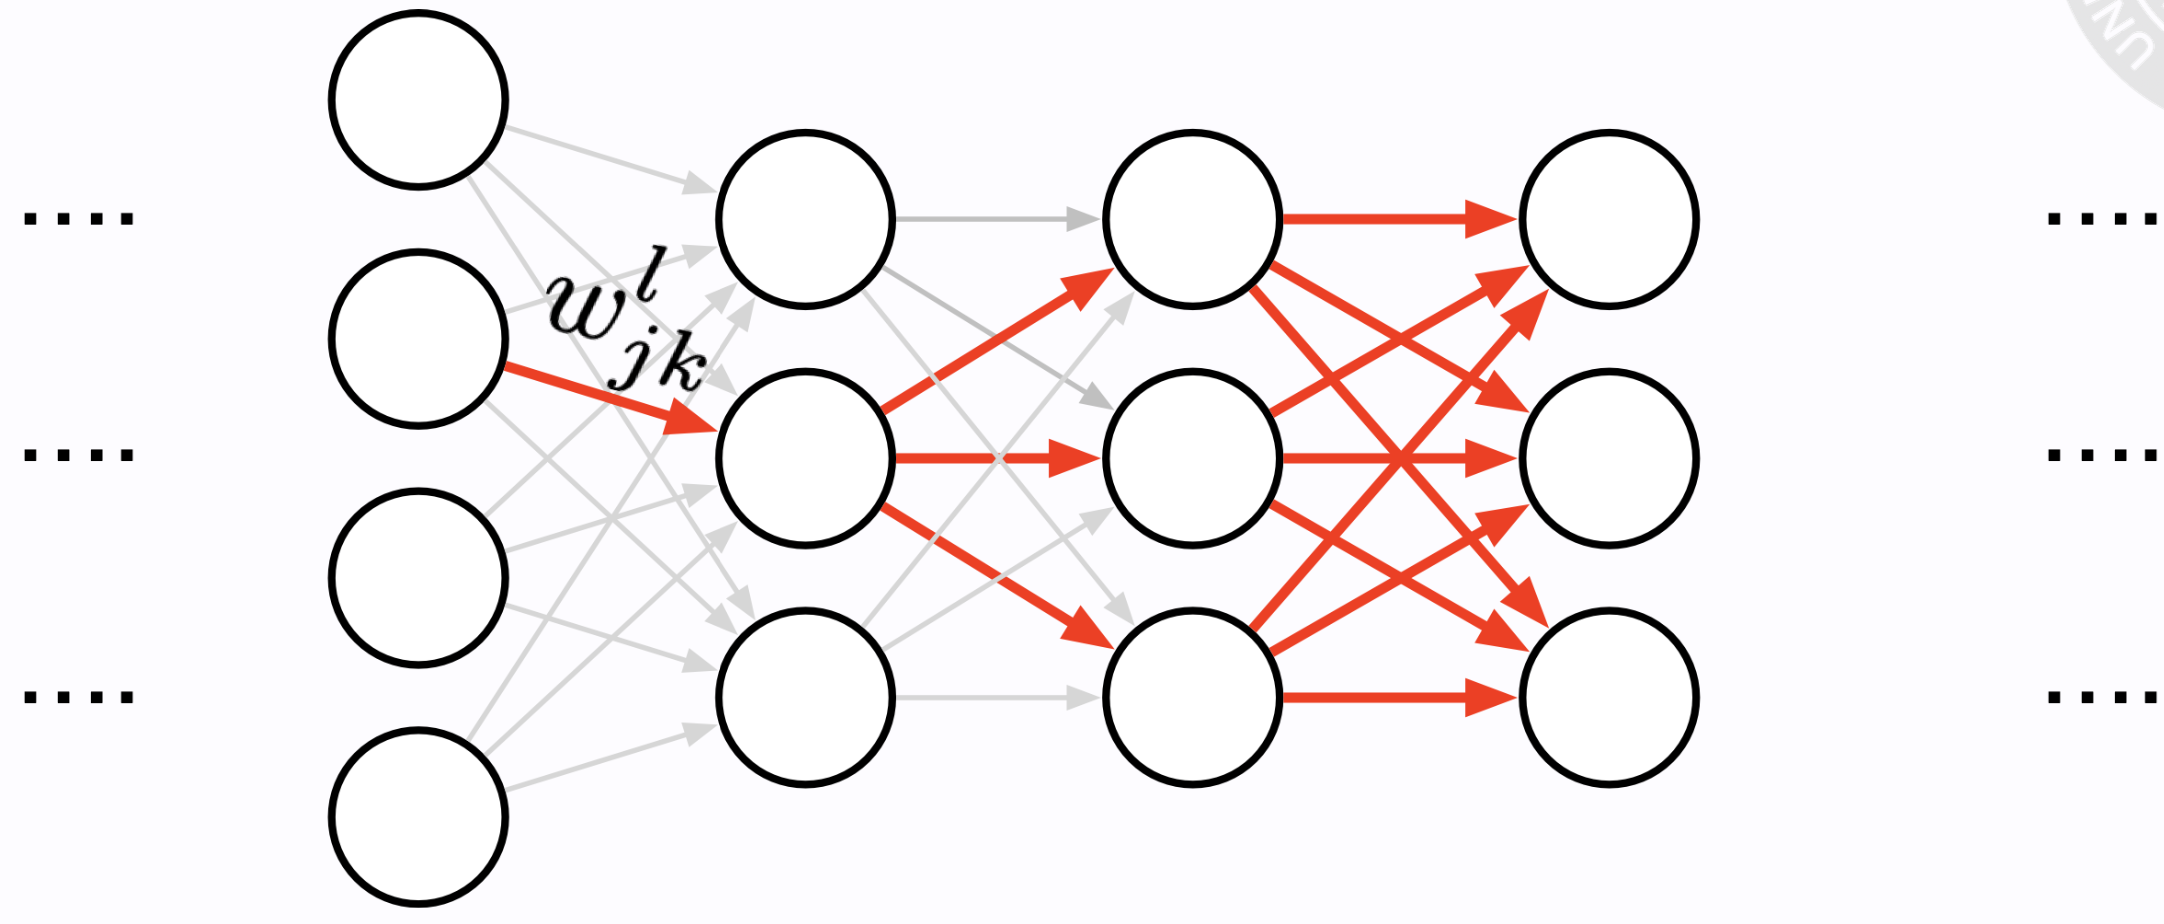
\includegraphics[scale=.44]{images/backpropagation/efficiency.png}
    \centering
\end{figure}
\newpage